\documentclass[11pt,a4paper]{article}

\usepackage[utf8]{inputenc}

\usepackage[spanish]{babel}

\usepackage{amsmath}

\usepackage{amsfonts}

\usepackage{amssymb}

\usepackage{makeidx}

\usepackage{xcolor}

\usepackage{multicol}

\usepackage{multirow}

\usepackage{graphicx}

\usepackage[left=2cm,right=2cm,top=2cm,bottom=2cm]{geometry}

\author{Eduardo Espuch}
\title{Apuntes de \emph{Matematicas 1}}
\date{}

\usepackage{fancyhdr}
\fancyhead[R]{curso 2018-2019}\fancyhead[L]{Apuntes de \emph{Matematicas 1}} \fancyfoot[C]{\thepage}
\pagestyle{fancy}



\begin{document}
\parskip=6pt
\maketitle

\begin{center}

\includegraphics[scale=0.6]{logoua}
\end{center}

\begin{abstract}
Documento que reune los conceptos dados junto con aclaraciones a lo largo de la asignatura de Matematicas 1. En el caso de que existe algun concepto externo que no se haya visto pero facilite el entender alguna explicacion, éste sera citado considerando que se ampliara la información en el anexo. 

Lo dire ya, deberia de verse antes el tema de matrices o verse juntos los sistemas lineales y las matrices, pero el temario esta dividido asi y se explican como el culo.
\end{abstract}


\begin{center}
\tableofcontents 
\end{center}
\newpage

\section{Introducción al álgebra lineal}

El algebra es una rama de las matematicas que estudia conceptos que podemos representar graficamente, es decir, los vectores (unidad mas sencilla), matrices y sistemas lineales (ambas estan correlacionadas y se componen de vectores, y espacios vectoriales (nuestra area de trabajo, nos ofrece los componentes y herramientas en forma de propiedades con las que operar) y sus transformaciones lineales. Hagamos una breve explicación para entenderlos mejor y poder relacionar los conceptos entre si (cabe destacar que esta no es parte del temario pero se ve necesario):

\begin{enumerate}
\item Vectores: elementos básicos de un espacio vectorial que unen dos puntos que se encuentran en el, sabemos ademas que todo espacio vectorial contiene al menos uno ya que por definicion este contiene al vector nulo, un punto en si. Los vectores se pueden entender como un polinomio, una funcion con varias incognitas (por lo general, estas incognitas ayudan a saber cuantas dimensiones posee un espacio vectorial ya que corresponden a los valores en cada eje. 

\item Sistemas lineales: conjunto de ecuaciones parametricas que pueden o no compartir soluciones para las incognitas, siendo esta la condicion principal para distinguir distintos tipos. Gráficamente se consideran un conjunto de rectas (ecuaciones de rectas y planos en el anexo) y los valores de las soluciones indican en que puntos se cruzan, las . Pueden realizarse operaciones entre las ecuaciones, debido a la combinacion lineal descrita en el espacio vectorial (se vera mas adelante)

\item Matrices: pueden verse como una reorganizacion de los sitemas lineales que actuan como un elemento de por si. Se definen operaciones y propiedades en particular para estos elementos y son de utilidad para relacionar sistemas lineales o para descomponerlos en sus partes basicas, las incognitas, sus coeficientes y los terminos independientes.

\item Espacio vectorial: la explicacion mas ampliada de este concepto se vera mas adelante pero bastara con saber que es una region de un determinado numero de dimensiones (cuantos ejes tiene, para entendernos) con la que estaremos trabajando en todo momento y estas descritas unas propiedades que consideraremos ciertas para todo momento (no es lo mismo trabajar en un espacio vectorial formado por los numeros reales que por el conjunto de numeros binarios, la suma convencional no tiene porque dar lo mismo en ambos casos pero ambas describirian un espacio vectorial).
\end{enumerate}

Los vectores y las ecuaciones de la recta no se consideran necesarias estudiarlas pero repasarlas no estaria mal. Hemos comentado que podemos clasificar los sistemas lineales segun la solucion para las incognitas o parametros (segun como interpretes cada ecuación las puedes llamar de una forma u otro pero son lo mismo al final), veamos que metodos de resolucion tenemos disponibles. Cabe destacar que, como ya se ha dicho, las matrices se pueden entender como SL reorganizados, por lo tanto se operara mucho con estas, se recomienda revisar el siguiente tema, al menos los conocimientos basicos de las matrices, para poder ir con soltura en las explicaciones (se indicara en negrita y cursiva cualquier concepto que consideremos sabido a partir de haber realizado dicha revision).

Segun el numero de soluciones, distinguimos:

\begin{enumerate}
\item Sistemas compatibles (o SL consistentes): aquellos sistemas en los que existe soluciones que relacionen las rectas. Si existen mas de una solucion hablaremos de un Sistema compatible indeterminado (SCI), donde estas soluciones definiran tramos de la recta en la que se sobreponen. Si es una unica solucion hablaremos de Sistemas compatibles determinados, donde se cruzan en un unico punto y no mas. Es mas, diremos que un SC es homogeneo si el termino independiente en todas las ecuaciones es 0 (una solucion trivial seria considerar las incognitas 0, llamaremos trivial a los procedimientos sencillos de obtener).

\item Sistemas incompatibles (SLI y no, no es la tecnologia de Nvidia para aparear tarjetas graficas): si no se encuentra ninguna solucion, las ecuaciones graficamente no se tocan, no existe relacion entre ellas alguna. 
\end{enumerate}

Entenderemos dos metodos de resolucion de SL, el directo y el iterativo, veamoslos:

\subsection{Resolucion de SL por metodos directos}

Usados para sistemas relativamente pequeños, los metodos directos consisten en aplicar un numero finito de pasos conocidos a priori con los que calcular la solucion exacta. No se recomienda realizar redondeo ya que estan sujetos a errar. Distinguimos 4 metodos al menos:

\subsubsection{Gauss y Gauss-Jordan}

Consideramos un Sistema lineal tal que:

$$\lbrace\begin{array}{c}
a_{11}x_1+a_{12}x_2+\dots+a_{1n}x_n=d_1\\
a_{21}x_1+a_{22}x_2+\dots+a_{2n}x_n=d_2\\
\vdots\\
a_{m1}x_1+a_{m2}x_2+\dots+a_{mn}x_n=d_m\\
\end{array}$$ donde $a_{ij}$ son los coeficientes para las $x_j$ incognitas y $d_i$ los terminos independientes correspondientes a cada operacion. Sabiendo los componentes de una sistema lineal, distinguirmos las siguientes matrices:
$$\left( \begin{array}{c c c c}
a_{11}&a_{12}&\dots&a_{1n}\\
a_{21}&a_{22}&\dots&a_{2n}\\
\multicolumn{4}{c}{\vdots}\\
a_{m1}&a_{m2}&\dots&a_{mn}\\
\end{array}\right)\left( \begin{array}{c}
x_1\\
x_2\\
\vdots\\
x_n\\
\end{array}\right)=\left( \begin{array}{c}
d_1\\
d_2\\
\vdots\\
d_m\\
\end{array}\right)\Leftrightarrow\left( \begin{array}{c c c c c}
a_{11}x_1&a_{12}x_2&\dots&a_{1n}x_n&d_1\\
a_{21}x_1&a_{22}x_2&\dots&a_{2n}x_n&d_2\\
\multicolumn{5}{c}{\vdots}\\
a_{m1}x_1&a_{m2}x_2&\dots&a_{mn}x_n&d_m\\
\end{array}\right)$$ o, mas simplifada, $Cx=D\Leftrightarrow A$ donde C es la matriz de coeficientes formada por $a_{ij}\in\mathbb{R}, \forall i,j\in\mathbb{N}$, x es la matriz de incognitas, D es la matriz de terminos independientes y A es la matriz ampliada que podemos escribir tambien como $[Cx|D]= A$.

Para resolver por Gauss y Gauss-Jordan se deben de obtener primero \textbf{\textit{la matriz escalonada}} y, en el caso de usar Gauss-Jordan, operarla con operaciones internas (llamalas combinaciones o transformaciones lineales, combinas dos ecuaciones) para obtener \textbf{\textit{la matriz reducida}}. Debido a que todo lo que se ha hecho hasta hora son combinaciones entre las ecuaciones, la matriz inicial (la ampliada en este caso) y las matrices escalonada y escalonada reducida son \textbf{\textit{matrices equivalentes}}, y por lo tanto los resultados obtenidos en unos son validos para los otros.

Ademas, si nos damos cuenta, estas matrices siguen siendo SL, con lo cual lo que estamos realmente haciendo es una sustitucion regresiva para despejar las incognitas. Si tenemos esto en mente el metodo de Gauss y Gauss-Jordan es muy util para despejar los sistemas compatibles (determinado si se nos da una unica solucion e indeterminado si una incognita depende de otra) o incompatible si vemos que dado el valor 0 para todas las incognitas (toda una fila de 0 en la matriz Cx escalonada/reducida) se un valor no nulo en la misma fila para los terminos independientes.

\subsubsection{Método de la inversa}

Habiendo visto lo que es una \textbf{\textit{matriz invertible}} y una \textbf{\textit{matriz inversa}}, ademas de saber que operando con matrices, \textbf{\textit{la matriz identidad}} es el elemento neutro en operaciones multiplicativas, el metodo de la inversa se basa en la siguiente propiedad:

Dado una matriz de coeficientes invertible C, una matriz de coeficientes x y una matriz de terminos independientes d, ya que $CC^{-1}=I$ y el sistema es Cx=d, podemos despejar la matriz incognitas de la siguiente forma:$$x=C^{-1}d\Leftrightarrow Ix=C^{-1}d\Leftrightarrow C^{-1}Cx=C^{-1}d$$

Es importante respetar las propiedades de operar con matrices y, obviamente, el conocer como despejar una matriz inversa, con lo cual se recomienda mirarse el tema siguiente.

\subsubsection{Descomposición LU}

Para entender este metodo de m... si o si necesitas mirarte el tema siguiente, miratelo... vuelve y ya hablamos porque vamos...

Metodo que requiere de que se den unas condiciones iniciales y de gran utilidad para despejar incognitas cuando se nos dan una gran variedad de matrices de terminos independientes para una misma matriz de coeficientes. Descompondremos la matriz de coeficientes en:

\begin{enumerate}
\item Matriz U, matriz escalonada de C en la que todos los elementos por debajo de la diagonal son 0 (matriz triangular inferior) y, si se obtiene intercambiando filas de posicion, este metodo ya no es valido. Se permite usar el siguiente tipo de combinacion $F_I\Leftrightarrow F_I+\lambda_{IJ} F_J$ y, ademas, sera importante dejar constancia de esto en la resolucion.

\item Matriz L, matriz cuadrada invertible (de tamaño en proporcion a la cantidad de elementos por debajo de la diagonal de U) que se obtiene a partir de poner en las posiciones(i,j) el $\lambda_{IJ}$ en negativo correspondiente. Veremos entonces que todos los elementos de la diagonal seran 1 y por encima de ella 0.
\end{enumerate}

Para llevar a cabo este metodo, lo que se hara, teniendo Cx=d, aplicaremos la igualdad C=LU obteniendo que LUx=d. Primero se obtendra un 'matriz de apoyo' y respecto a los terminos independientes Ly=d, siendo SCD resoluble por sustitucion progresiva. Lo siguiente sera obtener las incogntias correspondientes a los mismos terminos usando esta matriz de apoyo usando la igualdad Ux=y usando Gauss.

\subsubsection{Metodo de Rouche}

Esta se propone ya que es muy rapida y apenas necesitas realizar operaciones complejas, al menos se puede usar para saber que tipo de sistema lineal es. Consiste en considerar el rango (nº lineas (ya sean filas o columnas, por lo general filas) independientes entre si, es decir, que no son combinacion de otras dos) y el nº de incognitas. El rango lo podemos estudiar haciendo submatrices $M_{nxn}$ y calculando su \textbf{\textit{determinante}} con n$\leq$(nº filas o nº columnas(se coge el menor ya que esta sera el mayor rango posible)). 

Si todos los determinantes de una submatriz $M_{nxn}$ con un n en concreto dan 0, podemos afirmar que es de rango n-1 pero, si un solo determinante da distinto de 0, diremos que su rango es mayor o igual a n y probaremos con n+1. Por lo general se empieza estudiando el rango de la matriz de coeficientes y despues se prueba la ampliada intercambiando una de las columnas por la matriz de terminos independientes.

Las relaciones serian:
\begin{enumerate}
\item[SLI:] R(C)<R(A)
\item[SCD:] R(C)=R(A)=nº de incognitas
\item[SCI:] R(C)=R(A)<nº de incognitas
\end{enumerate}


\subsection{Resolucion de SL por metodos iterativos}

Metodo que resuelve un SL a base de partir de un caso inicial e ir probando si se aproxima a la solucion, no pierde tiempo en buscar como solucionarlo y haciendo los calculos necesarios para ello. Aunque parezca que no es muy practico, se nota su eficacia a la hora de trabajar con un numero muy elevado de variables y el realizar operaciones con semajante numero de incognitas seria complicado. Este metodo tiene unas ventajas (desde el punto de vista informatico) ante los metodos directos, son menos sensibles de errar en el redondeo y ademas, solo es necesario almacenar los valores no nulos del sistema.

Valiente h... de p... quien se vaya a ver esto, me esta dando mucha pereza el memorizar el algoritmo de jacobi

\section{Matrices}

Como necesitas definir algunas operaciones para poder obtener algunos tipos de matrices, dividiremos este tema de una forma alternativa a la del temario dado, dando primero conocimientos básicos (tipos de matrices básicas que no requieren de operaciones, operaciones entre matrices básicas,... todo lo que se pueda considerar necesario para conocer otro tipo de matrices), matrices compuestas (matrices obtenidas por distintas operaciones, acompañadas por operaciones mas avanzadas) y una breve recopilación de todas las matrices y funciones con una breve descripción.

\subsection{Conocimientos básicos}
Las matrices son conjuntos de elementos ordenados en n filas y m columnas tal que a cada elemento le corresponde una posicion, denotando a la matriz con mayusculas $A_{nxm}$ y al elemento $a_{ij}\in \mathbb{R}$ con $i\leq n,j\leq m$ siendo $n,m,i,j\in \mathbb{N}$. Llamaremos dimension de una matriz A a las dimension nxm de estas y rango de una matriz al numeros de filas o columnas linealmente independientes, es decir, que no sean una combinacion de otras dos.

Podemos distinguir muchos tipos de matrices ya sea por su forma (matrices fila, columna, rectangular,...) o sus elementos (nula, diagonal escalar o identidad, triangular,...) ademas de otras que son resultado directo de operaciones con matrices elementales (matriz escalonada, traspuesta, reducida,..). Las veremos por encima:
\begin{enumerate}
\item[·]Matrices fila y columna, tambien conocidas como vectores, son matrices en las que unicamente estas compuestas por una fila ($A_{1xm}$) o una columna ($A_{nx1}$).

\item[·]Matriz rectangular, matrices $A_{nxm},n\neq m$.

\item[·]Matriz cuadrada,  matrices $A_{nxn}$, tambien pordemos llamarlas amtrices de orden n. Son las matrices mas importantes para demostrar propiedades y las podemos clasificar como simetricas si $a_{ij}=a_{ji}$ o antisimetrica si $a_{ij}=-a_{ji}, i\neq j$ y $a_{ii}=0$ con $i,j\leq n$ siendo $n,i,j\in \mathbb{N}$.

\item[·]Matriz diagonal, matrices en las que todos los elementos salvos los de la diagonal ($a_{ii}$) son nulos. No importa si es rectangular, cuadrada, fila o columna, la diagonal se considera existente a partir del primer elemento de la matriz. Podremos llamarla diagonal escalar si todos los elementos de la diagonal son el mismo valor y, si ademas, este valor es el uno y la matriz es cuadrada, la llamaremos Matriz identidad, una matriz de gran utilidad.

\item[·]Matriz elemental, es una matriz identidad en la que se ha realizado una unica operacion correspondiente a la realizada en otra operacion. Estas matrices si se prefiere entender como matrices de registro de operaciones creo que sera mas comodo de recordar su funcion. Se dan tres operaciones: permutaciones (cambio de lineas), multiplicar una fila por un escalar y combinacion lineal (una linea es resultado de una operacion entre ella misma y otra acompañada por un escalar).

\item[·]Matriz triangular, son matrices en las que todos los elementos por encima o por debajo de la diagonal, no ambas a la vez, son nulos. Seran de triangular superior si los elementos nulos estan por encima y tirangular inferior si estan por debajo. Son de gran utilidad ya que se pueden dar para sustitucion progresiva y regresiva, respectivamente. No importa la forma.

\item[·]Matriz escalonada y reducida, son matrices triangulas inferiores que se obtienen a partir de otra matriz usando las operaciones de las matrices elementales. El elemento principal de una linea es el primer elemento que nos encontremos no nulos al recorrer dicha linea (ya sea fila o columna). En las matrices escalonadas se busca tener 1 principales en las filas y en la reducida 1 principales en las columnas (no siempre se podra, depende de que tipo de SL sea la matriz). Se pueden dar casos de que, si se trata de un SCD, una matriz escalonada reducida de el valor de cada incognita directamente.

\item[·] Las matrices equivalentes es la relacion existente entre una matriz y otra sobre la que se le han aplicado las operaciones de una matriz elemental (la matriz original por todas las matrices elementales(?)), por definicion las matrices escalonada y reducida son equivalente a su matriz original.

\item[·]Matriz traspuesta, matrices en las que se intercambian filas por columnas tal que el elemento $a_{ij}$ en la matriz normal es el elemento $a_{ji}$ en la traspuesta, obiamente en la diagonal no se vera cambio ni en las matrices simetricas.

\item[·]Submatriz o bloque de $A_{nxm}$, matrices que se obtienen al omitir alguna fila o columna de la matriz A. Es usada para estudiar matrices mas grandes por bloques y no importa la forma, pueden ser rectangulares o cuadradas. 

\end{enumerate}

Sabiendo ya las matrices basicas, veamos como trabajar con ellas:

\begin{enumerate}
\item[·] Operacion asociativa:

Las matrices integrantes deben de ser de las mismas dimensiones y los elementos en las mismas posiciones se suman. Se distinguen las propiedades asociativa (aislar operaciones por prioridad), conmutativa (cambiar el orden de prioridad), la existencia del elemento opuesto (un matriz y su opuesto dan matriz nula) y la existencia del elemento neutro (siendo el elemento neutro la matriz nula, al operar una matriz con esta el resultado vuelva a ser la matriz).

\item[·] Operacion multiplicativa: 

Se puede distinguir la multiplicacion de un escalar por una linea (operacion de las matrices elementales), un escalar por una matriz (todos los elementos de la matriz se multiplican por dicho escalar) o dos matrices. Para multiplicar dos matrices se tiene que el numero de columnas de la primera es igual al numero de filas de la segunda. La operacion consiste en dada una posicion en la matriz resultado, se realiza un prodcuto escalar escalar (o punto, como lo llaman aqui) de la fila correspondeinte de la primera por la columna correspondiente de la segunda traspuesta (fila por columna).

 Distinguimos que la conmutativa no existe, y si lo hace, diremos que esas matrices conmutan, no es simplificable (no existe cancelacion), se cumple la asociativa, la distributiva y existe el elemento neutro, que es la matriz identidad. Se puede tambien dar potencia de matrices al multiplicar las por si mismas y, ademas, estas son ciclicas, es decir, dado un numero finito de veces, el resultado de multiplicar tantas veces la matriz es la matriz identidad, ayudando a operar potencias elevadas.
 
\item[·]Determinante:

Es un escalar asociado a una matriz cuadrada. El metodo de obtenerlo varia pero todos son aceptados, se dajara un ejemplo a continuacion: 

\begin{tabular}{c c}
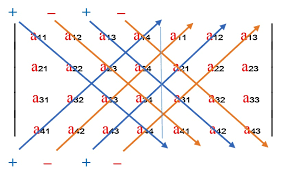
\includegraphics[scale=0.8]{d1}&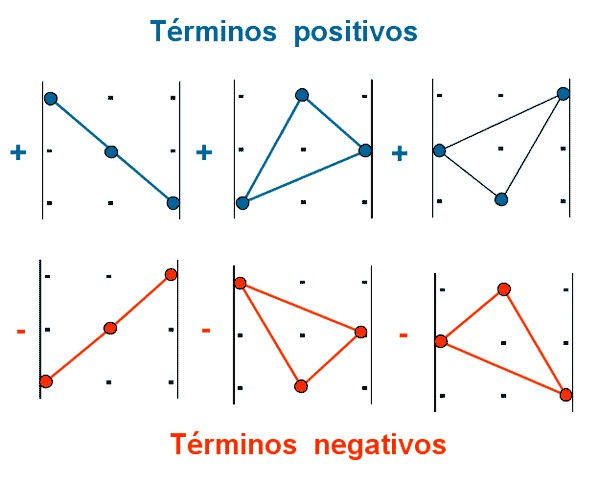
\includegraphics[scale=0.4]{d2}\\
La matriz se amplia&La matriz se mantiene\\
\end{tabular}

Cada linea es una operacion multiplicativa entre los terminos que la componen y se realiza una operacon asociativa con todas las lineas considerando el termino correspondiente.

 Se puede tambien obtener por los adjunto de una linea, siendo una suma de los elementos de una linea por su adjunto correspondiente.
 
 Los determinantes cumplen varias propiedades faciles de demostrar, el determinante de una matriz suma/producto es igual a la suma/producto de los determinantes de dicha matriz, al multiplicar una linea de la matriz por un escalar, el determiannte tambien se multiplica por este, la permutacion de lineas en una matriz puede cambiar el singo del determinante pero no el valor, si hay un vector nulo en la matriz, el determiante sera nulo y si una linea es combinacion de otras, el determinante es nulo.
 
 Usaremos los determinantes para estudiar rangos o para otro tipo de operaciones mas complejas.

 \item[·]Adjunto(no en el temario pero se adjuntara): 
 
 Sabiendo que el menor complementario de un elemento es el determinante que se obtiene se la submatriz en la que se omiten la fila y la columna en la que este elemento se encuentra, diremos que el adjunto a este elemento es el menor complementario por el signo correspondiente a su posicion ($(-1)^{i+j}$). Esta operacion se usara para obtener determinantes o para definir la matriz adjunta. 
 
\end{enumerate}


\subsection{Matrices compuestas}

Con los conceptos anteriores podemos definir:

\begin{enumerate}
\item[·] Matriz adjunta:

Matriz que se forma a apartir de los adjuntos de otra matriz.

\item[·] Matriz invertible:

Si dada una matriz cuadrada y un numero finito de matrices elementales (recordar que estas son matrices que registran una unica operacion en una matriz identidad), se cumple $AE_kE_{k-1}\dots E_2E_1=I$ diremos que la matriz A es invertible. Es mas, por definición, toda matriz elemental es invertible seguro ya que existe un inverso de este que permite obtener la identidad. 

En el caso de que no exista ninguna combinación en la que se obtiene I, hablaremos de una matriz singular. La inversa de la permutación es ella misma, la inversa de multiplicar una fila por un escalar es dividir y la inversa de sumar un elemento es restar. Entonces podemos también decir que $A=E_k^{-1}E_{k-1}^{-1}\dots E_2^{-1}E_1^{-1}I$
o lo que es lo mismo (ya que I es el elemento neutro podemos omitirlo) $A=(E_kE_{k-1}\dots E_2E_1)^{-1}\Leftrightarrow A^{-1}=E_kE_{k-1}\dots E_2E_1$ siendo $A^{-1}$ la matriz inversa de A y que por definición esta es también invertible y ademas $AA^{-1}=I$.

Se puede obtener de dos formas, con la demostrada multiplicando todas las matrices elementales necesarias para hacer A la matriz identidad (mucho mas rápida y sencilla) o con la matriz adjunta traspuesta partida el determinante.
\end{enumerate}

\section{Espacio vectorial}

Vamos a considerar que se conocen al menos que son los vectores y las operaciones descritas con ellos (escalar con cos y vectorial con sen), y sabiendo que una base la forman tantos vectores como la dimension con la que trabajamos y que estos sean no coplanarios, es decir, que no son combinaciones entre ellos, diremos que es ortogonal si estos vectores son perpendiculares, normal si son de modulo uno y ortnormal si las dos anteriores. Tambien sera necesario que -40ºC son -40ºF, es un dato de extrema importancia.

Siempre que hemos hablado de puntos y vectores en un espacio, hemos dado por entendido el concepto de espacio sin saber realmente en que consiste y porque podemos trabajar con estos elementos sobre el, veamoslo.

\subsection{Espacio y subespacio vectorial}

El espacio vectorial V y el subesapcio vectorial W tal que $W\subset V$, es decir, W es un subconjunto de elementos de V, son conjuntos de elementos expresados vectorialmente en V y W, respectivamente, en las que se definen una operacion interna suma(operan dos elementos del mismo conjunto) y una operacion externa multiplicativa(un elemento del conjunto dado opera con otro elemento externo a este conjunto, por lo general seran un conjunto de escalares). En la oepracion interna distinguimios la asociativa, distributiva, conmutativa y existencia del elemento neutro y opuesto y en la oepracion externa la asociativa, distributiva y el elemento neutro. 

(Fuera del temario) Para demostar que tanto el EV como el SEV son en si espacios vectorial, bastaria con probar que $\alpha \vec{u}+\beta \vec{v}\in V, \forall \vec{u},\vec{v}\in V, \alpha ,\beta \in \mathbb{E}$ siendo V el conjunto con el que trabajamos para estudiar si es EV y $\mathbb{E}$ un conjunto de escalares (puede ser el conjunto de numeros reales o algun subconjunto). Con esta demostracion se prueba que operando con elementos internos se puede dar otro elemento interno, es decir, que la combinacion lineal de elementos en EV pertenece, a su vez, a EV. Ademas, siempre que podamos definir un vetor nulo, podremos afirmar que es un EV ya que la demostracion es trivial.

Veamos algunos conceptos del espacio vectorial y recordemos que estos son aplicables al subespacio.

\subsubsection{Combinación lineal}

Se ha comentado el concepto de combinacion lineal anteriormente y este es facil de entender por contexto, pero veamos en que consiste. Dado un vector $\vec{v} \in \mathbb{R}^n$ donde n es la dimension del espacio vectorial de $\mathbb{R}$, y dada la siguiente igualdad $\vec{v}=\alpha_1\vec{u}_1+\alpha_2\vec{u}_2+\dots+\alpha_k\vec{u}_k=\sum_{i=1}^k\alpha_i\vec{u}_i$ donde $\vec{u}_i\in \mathbb{R}^n,\alpha_i\in \mathbb{R}$ con i=1,\dots ,k diremos que $\vec{v}$ es combinacion lineal (CL) para uno vectores $\vec{u}_i$ y unos escalares $\alpha_i$ dados.

 Se puede demostrar haciendo un SL y despejando  $\vec{v}=\alpha_1\vec{u}_1+\alpha_2\vec{u}_2+\dots+\alpha_k\vec{u}_k$ en los componentes cartesianos para obtener dicho SL. Si es SCD, existe una unica combinacion lineal para obtener este vector, si es SCI, existen varias opciones para obtener en vector $\vec{v}$ y si es SLI entonces este vector no es combinacion lineal de los vectores $\vec{u}_i$. Las incognitas suelen ser los escalares ya que se querra demostrar si unos vectores pueden obtener otro, con lo cual si realizamos un sistema matricial A=[Cx|D], C seran los escalares, x los vectores $\vec{u}_i$ y D el vector $\vec{v}$. En el caso de que sea SCD, diremos que que C y D son compatibles.

\subsubsection{Envoltura lineal}

Llamaremos envoltura lineal de V al conjunto de vectores con los que poder escribir todos los vectores de V, es decir, $\forall \vec{v}\in \mathbb{R}^n, \exists ! \vec{u}_1,\dots ,\vec{u}_n\in \mathbb{R}^3, \vec{v}=\alpha_1\vec{u}_1+\alpha_2\vec{u}_2+\dots+\alpha_n\vec{u}_n\text{ con }\alpha_i\in \mathbb{R}, i=1,\dots ,n$. Los vectores $\vec{u}_i$ sera vectores generadores o un subconjunto de $\mathbb{R}^3$ generador del espacio $\mathbb{R}^3$. Si dos elementos que forman una envoltura son combinacion lineal y lo demostramos, podremos omitir dicho elemento.

 Por lo general, el conjunto generador tendra tantos elementos como dimensiones tenga el espacio generado (una envoltura con un elemento define una linea, con dos eslementos un plano, con tres un espacio) aunque no tiene porque, si el conjunto y la envoltura coinciden, llamaremos base a esta envoltura ya que es el menor conjunto capaz de generan al conjunto.
 
Para demostrar que un conjunto es generador bastaria con probar que un vector cualquiera del conjunto generador es compatible con una unica combinacion de escalares, es decir, probar que es un SCD. Si fuese SCI, uno de los vectores generadores seria combinacion lineal de otro.
 
  Sera necesario saber que significa que unos vectores linealmente independientes y linealmente dependientes para poder hacer mas claras algunas explicaciones de demostracion.
  
  Un conjunto de vectores linealmente independientes son vectores que, la unica combinacion posible para obtener el vector nulo, seria que todos los escalares fueran ceros. Graficamente se observa que estan con el mismo angulo respecto a los demas (cuando haces un sistema de referencia, el ehe x, y y z son linealmente independientes).
  
  Un conjunto de vectores es linealmente dependiente si al menos uno de estos es combinacion lineal de otro, lo que resultaria en que, para obtener el vector nulo, existiria mas de una operacion. Se vera cuando queramos demostrar que un vector se puede omitir en una envoltura lineal, ya que si podemos definir un vector como combinacion de los otros, este operar con este seria sustituir un valor ya obtenido.
  
  Se estudia si es LD o LI usando un sistema lineal homogeneo.
  
  Las bases ya se han comentado por encima que son, vienen denotadas por letra caligrafica
y consiste en una envoltura lineal con conjunto de vectores estrictamente linealmente independientes entre si. En este caso, las dimensiones del espacio delimitaran el numero de vectores que lo definen. Una base no tiene que ser la unica que defina al conjunto generado, su demostracion seria tan sencilla como usar los multiplos de una base que sabemos que es cierta.

\subsection{Matrices y espacios vectoriales}

Solo por aclarar, aunque se puede observar con las explicaciones anteriores, las matrices se pueden entender como reordenaciones de los vectores de tal forma que, por lo general, las columnas son vectores y las filas son los componentes cartesianos en el mismo eje o dimension. Sabiendo esto, se pueden estudiar las relaciones entre los vectores usando un sistema matricial y comprobando si son SCD, SCI o SLI. 

Un resultado curioso es, si dada una matriz de vectores, la reducimos para obtener 1 principales, si nos da una matriz identidad, ese conjunto de vectores sabremos que es una base, si se da que es SCI, sera una envoltura lineal con un vector de mas y si es SLI pues caca, como si quieres decir que es lo de Nvidia, en este caso dices que son LD y sudas.

Para que no te confundas a la hora de reordenar los vectores, descomponelos a los componentes cartesianos, cada linea debe de agrupar en un sentido u otro a los componentes del mismo eje.

\section{Valores y vectores propios de una matriz}

Oh god dammit, alla vamos con el que si que puede ser un poco mas tedioso que la profesora de fc (mah bois pillaron la referencia). 

Dada una matriz A de orden n, un vector $\vec{v}$ en $\mathbb{R}^n$ y un escalar (real o complejo) $\lambda$, si se cumple la igualdad $A\vec{v}=\lambda \vec{v}\Leftrightarrow A\vec{v}-\lambda \vec{v}=0\Leftrightarrow A\vec{v}-\lambda I \vec{v}=0$ (esta ultima igualdad se obtiene por propiedades), diremos que $\lambda$ es un valor propio o autovalor y $\vec{v}$ es el autovector o vector propio asociado a este. Un autovector pero un autovalor puede tener muchos autovectores asociados a el (un autovector y los multiplos de este estan asociados al mismo valor propio). 

Los autovalores se pueden obtener con la ultima igualdad, que se puede entender como un sistema matricial tal que $A\vec{v}-\lambda I \vec{v}=(A-\lambda I)\vec{v}=0$ que sera un sistema homogeneo, si hacemos determinante de $(A-\lambda I)$y lo igualamos a 0 podemos obtener los autovalores que deben de ser distintos de ceros. Esta operacion recibe el nombre de polinomio caracterisitco $q_A(\lambda )=det(A-\lambda I)=0$, siendo cada raiz del polinomio un autovalor.

 El SH debera de ser SCI ya que, como se ha dicho, un autovalor puede estar asociado a muchos autovectores, por ejemplo sus multiplos. El conjunto de autovectores asociados a un autovalor se agrupan en el conjunto $E_A (\lambda )$, llamado autoespacio o espacio propio.

NOTA: Veamos ahora las matrices, que podemos sacar de ellas. Las matrices son bases de un espacio y los autovalores son los escalares que toman los vectores generadores para definir un vector, de ahi que un autovector se asocie a un solo autovalor pero no se cumpla el reciproco, porque en el primer caso, dado la base (la matriz) y el autovalor asociado es la unica combinacion posible para obtenerlo pero, un auto valor puede ser reusado para obtener mas vectores. Esta explicacion es de cosecha propia y creo que ayuda a entender que se hace pero como veais. Es mas, si reduces la tabla de tal manera que es una matriz diagonal, la diagonal te da los autovalores correspondientes a esta, lo que significa que en cada dimension el autovalor en dicha posicion es la que opera pra obtener el vector deseado. Es un poco abstracto pero si se pone a probarlo lo sacas. y OJO, el numero de autovalores corresponde al grado de autovalores que a su vez corresponde con las dimensiones del espacio.

En ocasiones, la ecuacion o polinomio caracteristico de A viene dado por raices, estas raices seran los posibles autovalores que pueden darse en dicha matriz y si se repite una misma raiz, entonces este autovalor tendra una multiplicidad algebraica equivalente al numero de repeticiones, viene denotado por ma($\lambda$). Llamaremos traza de A a la suma de todos los autovalores de esta (que casualmente coincidiria con la de las matriz escalonada reducida comentada en le NOTA anterior) y el determinante seria la multiplicacion de todas ella (CTRL+C, CTRL+V del parentesis anterior).

Dado un polinomio caracteristico, podemos calcular la inversa de la matriz asociada si sustituimos $\lambda$ por A y los terminos independientes vienen dados por la matriz I (Tº de Cayley-Hamilton).

 Los autovectores de dos autoespacios con autovalores distintos son linealmente independientes, y la base de estos autoespacio es cualquier autovector en el (demostracion clara con los multiplos). Llamaremos multiplicidad geometrica de $\lambda$ a la dimension del autoespacio asociado a $\lambda$ y se denota por mg($\lambda$). 
 
 Es un tema que parece sencillo pero es mucha teoria comprimida con lo cual se recomienda probar uno mismo el que se hare graficamente ya que, al final, tratamos con vectores y escalares reordenados.
 
 Alguna duda entrarme con @eduespuch (en insta igualito, para que me sigais) y se que he puesto que iba a hacer un anexo pero me da pereza y con esto es mas que suficiente.

\end{document}
\appendix
